\documentclass[a4paper,12pt]{article}

\title{Introduktion til programmering, ugeseddel 4}
\author{Version 1.0}% Martin Dybdal
\date{21.\ september 2014}

\usepackage[top=2cm,left=25mm]{geometry}
\usepackage[T1]{fontenc}
\usepackage[utf8]{inputenc}
\usepackage[danish]{babel}
\usepackage{cmap}
%\usepackage{microtype}
\hyphenpenalty=750

\usepackage{amsmath}
%\usepackage{lmodern}
%\usepackage{mathptmx}
%\usepackage{libertine}
%\usepackage[scaled=0.90]{inconsolata}
%\usepackage[scaled=0.83]{beramono}

\usepackage{enumerate}
\usepackage{listing}
\usepackage{fancyvrb}
\usepackage{graphics,tikz}
\usepackage{listings}
\usepackage{framed}
\usepackage{upquote}

\lstset{
    language=ML,
    keywordstyle=\bfseries,
    showstringspaces=false,
    basicstyle=\footnotesize\ttfamily,
    %numberstyle=\footnotesize,
    %numbers=left,
    %stepnumber=1,
    numbersep=10pt,
    tabsize=2,
    breaklines=false,
    aboveskip={0.7\baselineskip},
    columns=fixed,
    escapechar=@
%    extendedchars=true
% frame=single,
% backgroundcolor=\color{lbcolor},
}

\usepackage{todonotes}
\usepackage{hyperref}
\hypersetup{pdftitle={Introduktion til programmering, ugeseddel 4},
            pdfsubject={},
            pdfauthor={},
            pdfkeywords={rekursion, funktioner, lister, funktioner som værdier, højereordensfunktioner},
            pdfborder={0 0 0}}

\setlength{\parskip}{1ex}
\setlength{\parindent}{0pt}
\setlength{\parfillskip}{30pt plus 1 fil}

\makeatletter
\newcommand\footnoteref[1]{\protected@xdef\@thefnmark{\ref{#1}}\@footnotemark}
\makeatother

\begin{document}
\maketitle{}
Den fjerde undervisningsuge handler om \textit{brugerdefinerede
  datatyper}, \textit{abstraktion} og \textit{kombinatorisk
  søgning}. Derudover skal vi arbejde videre med lister, brug af
listekombinatorer og brug af funktioner som argumenter og
returværdier.


\subsubsection*{Omrokering:}
Vi bytter rundt på fredagsforelæsningen og mandagens
repetitionstime. Fredagen her i uge 4 vil derfor blive brugt på
repetition og begge timer mandag morgen i uge 5 vil dække nyt
stof.

En anden ændring er at vi har fordelt tirsdagsøvelserne mellem tirsdag
og fredag, så den første time begge dage bruges på at gennemgå øvelser
fra ugesedlen og den anden time bruges på at arbejde på
afleveringsopgaverne.

\section{Plan for ugen}
\label{sec:pensum-og-plan}

\subsubsection*{Mandag}
Simple indbyggede datatyper og brugerdefinerede datatyper

\textit{Pensum:} HR: 7.1-7.5

\subsubsection*{Tirsdag}
Abstraktion, brugerdefinerede undtagelser og kombinatorisk søgning

\textit{Pensum:} IP-2: 9 $\rightarrow$ HR: 7.6-7.7

\subsubsection*{Fredag}
Repetition af ugens pensum. Se ovenfor.

\newpage
\section{Mandagsopgaver}
\label{sec:mandagsopgaver}
\textit{Emner:} listekombinatorer, anonyme funktioner og \lstinline{option}-datatypen

\begin{enumerate}[{4}M1]
\item Definer en anonym funktion der sætter paranteser om en
  \lstinline{string}. Anvend den anonyme funktion på alle elementerne
  i listen \lstinline{["a", "b", "c", "d"]}.
\item Brug \lstinline{ListPair.zip} og \lstinline{map} til at skrive en funktion
\begin{lstlisting}
  differences : int list -> int list
\end{lstlisting}
  Sådan at kaldet:
\begin{lstlisting}
  differences [x@$_1$@, x@$_2$@, x@$_3$@,@$\ldots$@,@x$_n$@]
\end{lstlisting}
  returnerer en liste der indeholder differencer mellem par af
  elementer i \lstinline{xs}.
\begin{lstlisting}
  [x@$_2$@-x@$_1$@, x@$_3$@-x@$_2$@, x@$_4$@-x@$_3$@,@$\ldots$@,@x$_{n}$@-x@$_{n-1}$@]
\end{lstlisting}

\item Her er \lstinline{lookup}-funktionen fra mandags-forelæsningerne
  i Uge 3:
\begin{lstlisting}
  (* lookup : (''a * 'b) list -> ''a -> 'b *)
  fun lookup []          key = raise Fail "Not in list"
    | lookup ((a,b)::xs) key = 
        if key = a then b
        else lookup xs key
\end{lstlisting}
Omskriv \lstinline{lookup} så dens returtype er \lstinline{'b option}

\item HR 7.2

\item Brug \lstinline{foldr} til at skrive funktionen
\begin{lstlisting}
  somes : ('a option) list -> 'a list
\end{lstlisting}
  der tager en liste af \lstinline{option}'s og returnerer listen af
  alle \lstinline{SOME}-værdierne.

\item Brug \lstinline{foldl} til at finde den største fællesdivisor
  for en liste af tal (Benyt at $0$ er neutral-element for \lstinline{gcd})

\item Vi har set at funktioner af to argumenter kan skrives på to måder:
  \begin{description}
  \item[Brug af tupler] \lstinline{'a * 'b -> c}
  \item[Sekventialiseret] \lstinline{'a -> 'b -> c}
  \end{description}
  
  Skriv funktionerne \lstinline{curry} og \lstinline{uncurry}, der
  konverterer mellem de to:

\begin{lstlisting}
  curry   : ('a * 'b -> c) -> ('a -> 'b -> c)
  uncurry : ('a -> 'b -> c) -> ('a * 'b -> c)
\end{lstlisting}

 (En anden forklaring af opgaven findes som opgave 9.5 i HR)
\end{enumerate}

\newpage
\section{Tirsdagsopgaver}
\label{sec:tirsdagsopgaver}
\textit{Emner:} Sortering, \lstinline{order}-datatypen og brugerdefinerede datatyper.

Det forventes, at du inden øvelserne tirsdag har forberedt dig på
opgaverne ved at løse så mange som muligt på egen hånd.
\begin{enumerate}[{4}T1]
\item Definer en datatype
\begin{lstlisting}
  datatype solution = ...
\end{lstlisting}
  der kan repræsentere de forskellige muligheder når der findes rødder
  i en andengradsligning: Ingen reelle rødder, én reel rod eller to
  reelle rødder.

Løs opgave 1G1 sådan at \lstinline{solve2} får typen
\begin{lstlisting}
  solve2 : real * real * real -> solution
\end{lstlisting}
Afprøv funktionen med samme kald som i 1G2 og 1G3.

\item Datatypen \lstinline{shape} i HR kapitel 7 kan udvides så alle
  shapes også har en placering i et todimensionelt koordinatsystem:
\begin{lstlisting}
  datatype point = Point of real * real
  datatype shape = Circle   of point * real
                 | Square   of point * real
                 | Triangle of point * real * real * real
\end{lstlisting}
  Skriv en funktion \lstinline{translate (x,y) shape} sådan at
  koordinaterne for cirklen, kvadratet og trekanten flyttes med
  vektoren \lstinline{(x,y)}. F.eks. skal funktionskaldet:
\begin{lstlisting}
  translate (-2.0,3.0) (Circle((0.0,1.0)), 5.0)
\end{lstlisting}
  returnere \lstinline{Circle((-2.0,4.0), 5.0)}.

\item  
De rationelle tal, er de tal vi kan skrive som en brøk af to
heltal:
\begin{lstlisting}
  datatype rational = Ratio of int * int
\end{lstlisting}
For eksempel kan brøkken $\frac{1}{3}$ repræsenteres som
\lstinline{Ratio (1,3)}.

Definer funktionen:
\begin{lstlisting}
  rationalCompare : rational * rational -> order
\end{lstlisting}
sådan at kaldet \lstinline{rationalCompare(a,b)} sammenligner to
rationelle tal og returnerer \lstinline{LESS}, \lstinline{EQUAL} eller
\lstinline{GREATER} afhængigt af om \lstinline{a} er mindre, lig eller
større end \lstinline{b}. 

Start med at forlænge brøkkerne, så de får samme nævner. Brug
\lstinline{lcm} til at finde det mindste fælles multiplum, der skal
bruges til at forlænge med.

\begin{lstlisting}
  (* Least common multiple *)
  fun lcm (n, m) = (n * m) div gcd(n, m)
\end{lstlisting}

\item Benyt rationalCompare og Listsort.sort til at sortere en liste
  af rationelle tal.
\end{enumerate}

\newpage
\section{Fredagsopgaver}
\label{sec:tirsdagsopgaver}
\textit{Emner:} Funktioner som værdier

Det forventes, at du inden øvelserne fredag har forberedt dig på
opgaverne ved at løse så mange som muligt på egen hånd.
\begin{enumerate}[{4}F1]
\item Funktionen \lstinline{quicksort} fra IP-2 afsnit 8.5 kan kun
  sortere lister af \lstinline{real}'s. Omskriv \lstinline{quicksort}
  til en polymorf funktion:
\begin{lstlisting}
  qsort : ('a * 'a -> order) -> 'a list -> 'a list
\end{lstlisting}

  Sådan at \lstinline{qsort} sorterer en liste ved brug af en
  sammenligningsfunktion, der er givet som parameter
  (f.eks. \lstinline{Int.compare} eller \lstinline{rationalCompare})

Quicksort fra IP-2, afsnit 8.5 til kopiere ind og arbejde videre på:
\begin{lstlisting}[basicstyle=\scriptsize\ttfamily,escapechar=£]
fun partition (_,[]) = ([],[])
  | partition (pivot : real, x :: xr)
    = let val (xv, xh) = partition (pivot, xr)
      in if x <= pivot then (x :: xv,     xh)
                       else (     xv,x :: xh)
      end
fun quicksort [] = []
  | quicksort (x :: xr)
    = let val (xv, xh) = partition (x, xr)
      in quicksort xv @ x :: quicksort xh end
\end{lstlisting}

\item Definer funktionen:
\begin{lstlisting}
  splitWhen : ('a -> bool) -> 'a list -> 'a list * 'a list
\end{lstlisting}
  sådan at et kald \lstinline{splitWhen p xs} opdeler \lstinline{xs}
  i to lister \lstinline{(ys, zs)} ved det første \lstinline{x} i
  \lstinline{xs} hvor \lstinline{p(x) = true}. Det skal gælde at
  \lstinline{xs = ys @ zs} og \lstinline{x} skal være det første
  element i \lstinline{zs}.

\item Benyt \lstinline{splitWhen} til at definere funktionen:
\begin{lstlisting}
  fields : string -> string list
\end{lstlisting}
  sådan at \lstinline{fields str} opdeler teksten \lstinline{str} i
  felter ved hvert komma. F.eks. skal kaldet \lstinline{fields ",foo,bar,baz,"} 
  returnere værdien \lstinline{["","foo","bar","baz",""]} og 
  kaldet \lstinline{fields "test"} returnere værdien \lstinline{["test"]}.
\end{enumerate}

\newpage
\section{Opgavetema: klavernoder}
I det vestlige tonesystem benyttes 12 toner:

\quad C, Cis, D, Dis, E, F, Fis, G, Gis, A, Ais og B\footnote{Tonerne
  har forskellige navne i forskellige skalaer, f.eks. har tonen Fis
  også navnet Ges, men det skal vi ikke bekymre os om her. Hvis der er
  musikere blandt de studerende, så kan I se det som om vi bygger et
  system der kun kan bruges til at skrive melodier i den kromatiske
  C-skala. Anse det som en forenkling foretaget af
  pædagogiske grunde}.

Vi kan repræsentere de tolv toner med denne datatype (enumeration):
\begin{lstlisting}
  datatype pitchclass = C | Cis | D | Dis | E | F | Fis
                      | G | Gis | A | Ais | B
\end{lstlisting}
\vspace{-8mm}
\begin{figure}[h!]
  \centering
  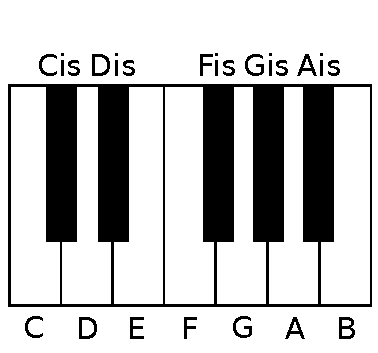
\includegraphics[height=8em]{uge4_oktav.pdf}
  \caption{En oktav på et klaver}
  \label{fig:oktav}
\end{figure}

På et klaver gentages disse tolv toner igen og igen i et antal
oktaver, hvor de oktaver der ligger til venstre for midten giver dybe
toner og de oktaver der ligger til højre for midten giver lyse (eller
"`høje"') toner.

Tonehøjden kan angives ved et tal der indikerer oktaven, vi vil bruge
0 til at indikere den midterste oktav og positive og negative tal til
at angive antallet af oktaver væk fra midteroktaven. Dette er
illustreret på følgende figur:
\begin{figure}[h!]
  \centering
  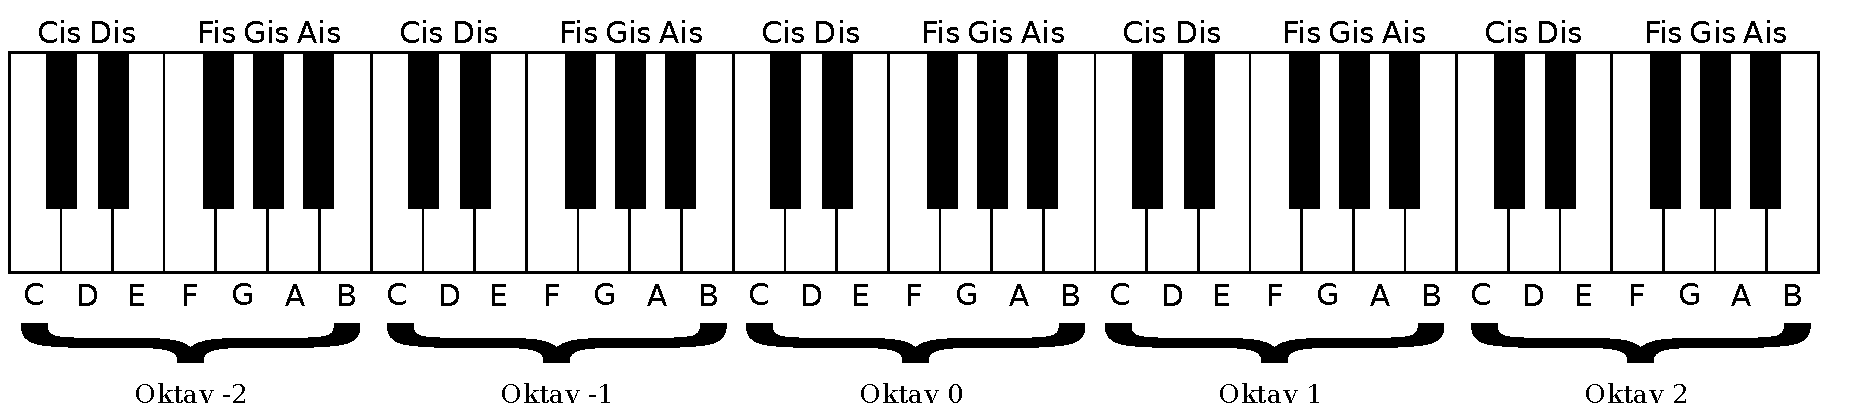
\includegraphics[width=\textwidth]{uge4_5oktaver.pdf}
  \caption{Et klaver med 5 oktaver}
  \label{fig:oktav}
\end{figure}

Vi kan nu definere:
\begin{lstlisting}
  type octave = int
  type pitch = pitchclass * octave
\end{lstlisting}

Den længste node man kan notere er \textit{helnoden}. Alle andre noder
og pausers varighed angives \textit{relativt} i forhold til varigheden
af en \textit{helnode}. På den måde kan tempoet af en sang justeres ved at angive
længden af en helnode og så følger længden af alle andre toner med. 

En tone der spiller i en fjerdedel af en helnode har længden $1/4$, vi
nøjes dog med at repræsentere varigheden som et heltal $d$, der er
nævneren i brøkken $1/d$. Vi repræsenterer altså varigheden af en
fjerdedelsnode med heltallet $4$ og varigheden af en helnode med
heltallet $1$.
\begin{lstlisting}
  type duration = int
\end{lstlisting}

En melodi kan nu beskrives ved angivelse af en liste af toner og
pauser, hvor der for hver tone er angivet længden tonen skal holdes og
en tonehøjde (oktav), og der for hver pause er angivet en længde af
pausen:
\begin{lstlisting}
  datatype music = Note of duration * pitch
                 | Rest of duration

  type melody = music list
\end{lstlisting}

\section{Gruppeaflevering}
\label{sec:gruppeaflevering}
Gruppeafleveringen obligatorisk.  Alle delspørgsmål skal besvares.
Opgaven afleveres i Absalon.  Der afleveres en fil pr.\ gruppe, men
den skal angive alle deltageres fulde navne i kommentarlinjer øverst i
filen. Filens navn skal være af formen
\texttt{4G-\textit{initialer}.sml}, hvor initialer er erstattet af
gruppemedlemmernes initialer. Hvis f.eks. Bill~Gates, Linus~Torvalds,
Steve~Jobs og Gabe~Logan~Newell afleverer en opgave sammen, skal filen
hedde \texttt{4G-BG-LT-SJ-GLN.sml}. Brug gruppeafleveringsfunktionen i
Absalon.

Gruppeopgaven giver op til 2 point, som tæller til de 20 point, der
kræves for eksamensdeltagelse.  Genaflevering kan hæve pointtallet fra
første aflevering med højest 1 point, så sørg for at gøre jeres bedste
allerede i første aflevering.

\begin{enumerate}[{4G}1]
\item Skriv en funktion \lstinline{musicToString : music -> string}
  der der konverterer en tone eller en pause til følgende format, der
  både er læsbart for mennesker og computere:

  \begin{itemize}
  \item Pauser printes som "`\lstinline{r}"' ("`r"' for
    "`rest"') efterfulgt af længden af pausen. En pause af en
    fjerdedels længde printes \lstinline{r4}. En pause af en
    toogtredivtedels længde printes \lstinline{r32}.
  \item Toner i midteroktaven (oktav 0) printes som tonensnavn (med
    lowercase) efterfulgt af længden af tonen. F.eks. printes
    \lstinline{Note (4, (Cis, 0))} som \lstinline{cis4} og
    \lstinline{Note (32, (B, 0))} som \lstinline{b32}.

    Toner i oktaver over eller under midteroktaven bruges et antal
    kommaer eller apostrofer\footnote{Apostroftegn er \lstinline{'},
      og ligger på tasten til højre for "`Ø"' på et dansk tastatur}
    til at angive oktaven. En apostrof går en oktav op og et komma går
    en oktav ned. \lstinline{Note (4, (Fis, 2))} udskrives som
    \lstinline{fis''4} og \lstinline{Note (1, (A, ~3))} som \lstinline{a,,,1}. 
  \end{itemize}

  Opdel problemet i passende delproblemer og skjul hjælpefunktionerne
  i en lokal erklæring.

\item Skriv en funktion \lstinline{melodyToString : melody -> string} der
  printer en hel melodi ved at kalde \lstinline{musicToString} for
  alle toner og pauser og indsætter et blanktegn mellem hver. Teksten \lstinline{"a16 b16 c'4 c'8"} bør returneres ved kaldet:
\begin{lstlisting}
  melodyToString [Note (16, (A,0)), Note (16, (B,0)),
                  Note (4, (C,1)), Note (8, (C,1))]
\end{lstlisting}

\item Nogle beregninger er nemmere at lave med en anden
  repræsentation, hvor hver en tone er angivet som et tal der angiver
  afstanden fra det midterste C på klaveret. 

\begin{figure}
  \centering
  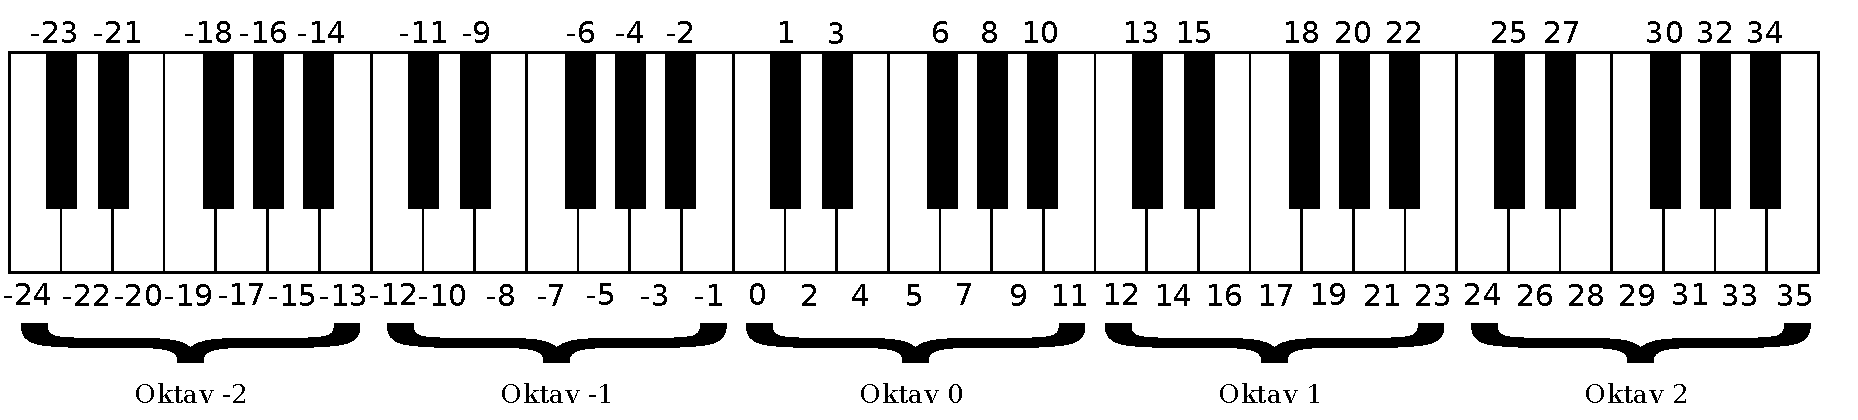
\includegraphics[width=\textwidth]{uge4_5oktaver_nummereret.pdf}
  \caption{Et klaver med 5 oktaver, hvor hver tangent er nummereret}
  \label{fig:oktav}
\end{figure}


\begin{lstlisting}
  type abspitch = int
\end{lstlisting}

Skriv en funktion \lstinline{absolutePitch : pitch -> abspitch}, der
kombinerer pitchclass og oktav i et enkelt tal. F.eks. skal
\lstinline{absolutePitch (A, ~1)} returnere \lstinline{~3} og kaldet
\lstinline{absolutePitch (G, 1)} skal returnere \lstinline{19}. Se nummerering
for et 5-oktavers klaver på Figur \ref{fig:oktav}.

\item Skriv en funktion \lstinline{pitch : abspitch -> pitch} der foretager den
  modsatte konvertering: fra et heltal til et par bestående af tone og
  oktav.

\item En melodi kan flyttes op eller ned et antal tonetrin, ved at
  flytte alle toner det samme antal skridt i samme retning. Dette
  kaldes at "`transponere"'.  Skriv funktionen
\begin{lstlisting}
  transpose : int -> melody -> melody
\end{lstlisting}
  sådan at \lstinline{transpose n mel} flytter alle tonerne i melodien
  \lstinline{mel} op eller ned med \lstinline{n} skridt (negativt
  \lstinline{n} betyder at tonerne skal transponeres ned).  Pauser
  skal bevares som de er.

  For eksempel skal kaldes \lstinline{transpose 3 [Note (32, (A,-1))]}
  returnere \lstinline{[Note (32, (C,0))]} fordi tre skridt over A
  (oktav -1) ligger C (oktav 0). Kaldet \lstinline{transpose ~12 mel}
  transponere melodien \lstinline{mel} ned med én oktav.

\item Skriv en funktion \lstinline{maxPitch : melody -> pitch}. Der
  finder den højeste tone i en melodi. Hvis listen er tom eller der
  kun er pauser i en melodi kastes undtagelsen \lstinline{Domain}.

\item Skriv en funktion \lstinline{duration : melody -> rational}, der
  udregner længden af en melodi i antal helnoder. Da vi ikke kan være
  sikker på at der samlet set er et helt antal af helnoder, skal
  funktionen returnere varigheden som en rationel værdi (se
  tirsdagsøvelserne, find evt. den vejledende løsning på Absalon).
\end{enumerate}


\newpage
\section{Individuel aflevering}
\label{sec:indiv-aflev}
Den individuelle opgave er obligatorisk.  Alle delspørgsmål skal
besvares.  Opgaven afleveres i Absalon som en fil med navnet
\texttt{4I-\textit{navn}.sml}, hvor \texttt{\textit{navn}} er
erstatttet med dit navn. Hvis du fx hedder Anders~A.~And, skal
filnavnet være \texttt{4I-Anders-A-And.sml}. Skriv også dit fulde navn
som en kommentar i starten af filen.

Den individielle opgave giver op til 3 point, som tæller til de 20
point, der kræves for eksamensdeltagelse.  Genaflevering kan hæve
pointtallet fra første aflevering med højest 1 point, så sørg for at
gøre dit bedste allerede i første aflevering.

\begin{enumerate}[{4I}1]
\item Betragt datatypen:
\begin{lstlisting}
  datatype ('a, 'b) either = Left of 'a | Right of 'b
\end{lstlisting}

Skriv funktionen
\begin{lstlisting}
  partEither : (('a,'b) either) list -> 'a list * 'b list
\end{lstlisting}
sådan at \lstinline{partEither xs} opdeler listen \lstinline{xs} i to
lister, hvor den første har alle \lstinline{Left}-værdierne og den
anden indeholder alle \lstinline{Right}-værdierne, i samme rækkefølge
som de optræder i den oprindelige liste.

\item Betragt datatypen:

\begin{lstlisting}
  type username = string
  type message = int * username * string
  datatype status = Online | Away | Offline
  datatype chatuser = User of username * status
  datatype chatroom = PrivateChat of username * message list
                    | GroupRoom of username list * message list;
\end{lstlisting}
  En bruger i en Chat-klient har et \textit{brugernavn} og en
  \lstinline{status}-angivelse (Online, Away, Offline). Der kan ikke
  være flere brugere med samme brugernavn.

  Chat-klienten understøtter både fler-bruger chatrum og private
  chatrum. For hvert chatrum er en liste af beskeder. En besked
  indeholder et brugernavn, en besked og en tidsangivelse
  repræsenteret som antal sekunder siden 1. Januar 1970 kl. 00:00:00.

\begin{lstlisting}
  val userlist = [User ("Sus", Offline), User ("Mike", Offline),
                  User ("Markus", Online), User ("Emil", Online)]
  val room = [PrivateUser ("Sus", [(793980034, "Sus", "Hello!")]),
              GroupRoom (["Mike", "Markus", "Emil"],
                         [(793983657, "Mike", "Hopla!")])]
\end{lstlisting}

  Skriv funktionen \lstinline{removeOffline : chatuser list * chatroom list -> chatroom list} 
  der fjerner de chatrum hvor alle brugere er \lstinline{Offline}.

\item Skriv en funktion der finder tidspunktet $t$ for den seneste
  besked i et chatrum og returnerer some $t$ (hvor $t$ er angivet i
  antal sekunder siden 1. Januar 1970 00:00:00), og returnerer NONE
  hvis der endnu ikke er skrevet noget i chatrummet.
\begin{lstlisting}
  newestMessage : chatroom -> int option
\end{lstlisting}

\item Skriv en funktion der sorterer en liste af chatrum efter hvornår
  der sidst har været aktivitet, forrest i listen skal alle chatrum
  uden aktivitet stå og derefter kommer chatrummene med senest
  aktivitet.
\begin{lstlisting}
  sortRooms : chatroom list -> chatroom list
\end{lstlisting}
\end{enumerate}


%\newpage
\section{Ugens nød}
\label{sec:ugens-nod}
I det følgende repræsenteres et punkt som to heltal:
\begin{lstlisting}
  type point = int * int
\end{lstlisting}

Følgende funktion kan bruges til at tegne ensfarvede \textit{figurer}
oven på et InstagraML-billede, hvor en \textit{figur} angives som en
funktion af typen \lstinline{point -> bool} der returnerer
\lstinline{true} ved de pixels der skal farves og \lstinline{false}
ved de farver hvor det underliggende billede skal bevares:
\begin{lstlisting}
(* Draw a figure (f) on top of an image (img) in
 * the specified colour. *)
fun drawFigure colour img f = 
  let val (w,h,f) = InstagraML.toFunction img
      fun overlay p = if f p then colour else f p
  in InstagraML.fromFunction (w,h, overlay)
  end
\end{lstlisting}

For eksempel kan en cirkel eller et rektangel tegnes ved at skrive
funktioner der afgører om et punkt er inde eller uden for figuren:
\begin{lstlisting}
(* Create a circle from radius and center point
     circle : point * int -> point -> bool
 *)
fun circle ((a,b), r) = fn (x,y) =>
  let fun square x = x*x
  in square (x-a) + square (y-b) < r end

(* Create a rectangle from its top left corner
   and its bottom right corner
     rectangle : point * point -> point -> bool *) 
fun rectangle ((x1,y1),(x2,y2)) = fn (p1,p2) => 
  Int.min (x1,x2) <= p1 andalso p1 <= Int.max(x1,x2) andalso
  Int.min (y1,y2) <= p2 andalso p2 <= Int.max(y1,y2)
\end{lstlisting}

\begin{enumerate}[{4N}1]
\item Skriv en funktion der afgører om et punkt er inde i et polygon
  eller udenfor, hvor et polygon er repræsenteret som en liste af
  punkter: \lstinline{point list}, sådan at den kan bruges til at
  tegne polygoner med \lstinline{drawFigure}.

  Benyt at du kan finde ud af om et punkt $(p_x, p_y)$ er på venstre
  side eller højre side af et linjesegment fra $(v_x, v_y)$ til $(u_x,
  u_y)$ ved at kigge på fortegnet af determinanten:
  \begin{equation*}
    \left|
      \begin{array}{ll}
        u_x-v_x & p_x-v_x \\
        u_y-v_y & p_x-v_y
      \end{array}
    \right|
  \end{equation*}
\end{enumerate}

\end{document}

%%% Local Variables:
%%% mode: latex
%%% TeX-master: t
%%% End:
